
\title{15-440: Lab 3}
\author{
        Spencer Barton (sebarton)\\
        Emma Binns (ebinns)
}
\date{November 18, 2014}

\documentclass[12pt]{article}

\usepackage{graphicx}
\usepackage[compact]{titlesec}
\usepackage[letterpaper, portrait, margin=1in]{geometry}
\usepackage{amsmath, amsfonts, amsthm, amssymb}

\newcommand{\ttt}{\texttt}

\setlength{\parindent}{0pt}
\setlength{\parskip}{\baselineskip}

\begin{document}
\maketitle

%------------------------------------------
\pagebreak
\section{Running the Framework}

\subsection{System Requirements}

MapReduce runs on a unix cluster. The CMU unix cluster will work. Place the code in a file on AFS as we rely on that file system to share all of our code files between participants.

\subsection{Set-up}

The following steps must be followed for a successful set-up.

\begin{enumerate}
\item 
Run \ttt{python SETUP.py} in the \ttt{src} directory. This will compile all of the code.

\item
Start participants: Connect with all machines that you wish to run participants on. Run \ttt{java participant\\Participant} from the \ttt{src} directory. If this does not work you may need to use the non-default port. Try running with the optional port argument \ttt{java participant/Participant <port>}. If you see the message \ttt{File server ran into trouble} then the file server is unable to run on that machine so try running the participant on anther machine or adjust the file server configuration file (see below note). An important note is that participants must run on different machines.

\item
Once you have some participants running, you will need to update the config file to point to these participants. Example config files can be found at \ttt{src/examples/ wordcount/wordcount.config} and \ttt{src/examples/wordoccurences/wordoccurences.config}. The key lines to modify, if you plan to run the examples, are \ttt{PARTICIPANT} and \ttt{NUM\_REDUCERS}. The \ttt{PARTICIPANT} values is \ttt{<hostname>:<port>}. When you started the participants there was a message to tell you which port it is running on.

\item
You are now ready to start the master. Pick a machine that does not have a participant running on it. Run \ttt{java master/Master} from the \ttt{src} directory.

\item
The master is now running. You will have a number of possible commands to enter to run jobs. See the next section for details.

\end{enumerate}

In addition to the configuration files mentioned above there is a file server configuration file to tell master and participants where remote files should be served from as well as which port the file server is running on. If you run into file permission issues or unavailable ports this configuration file can be found at \ttt{fileIO/fileserver.config}. Make sure that the specified directory is not in AFS as that would cause conflicts as files move around.

\subsection{Manage a Job}

Now that you have the master and participants running you are ready to start a job. The master provides a command line interface to type three possible commands.

\begin{itemize}
\item
\ttt{start <path\_to\_config\_file>} This will start a process and print results as the process goes. It will also print the process id (PID) for your use with other commands. (Ex  \ttt{start src/examples/wordcount/wordcount.config})

\item
\ttt{stop <pid>} Stops the specified process

\item
\ttt{status <pid>} Gets the status of the specified process

\end{itemize}

%------------------------------------------
\section{For the Application Developer}

\subsection{Writing Your Map-Reduce Functions}

We provide two interfaces to which the application developer must adhere. The first is \ttt{MapFn} which requires a \ttt{map(String input) -> MRKeyVal(String key, int value)} method. This method takes strings which are the lines of the input file and maps them to a key-value pairs where keys are strings and values integers. If \ttt{map} returns \ttt{null} then the mapper framework will ignore the result.

The second interface is \ttt{ReduceFn} which requires a \ttt{reduce(String key, List<int> values) -> MRKeyVal(String key, int value)} method. This method takes a key and all of the values that had that key and returns a reduced result on the values in the form of a single key-value pair. If this method returns \ttt{null} then the result is ignored.

\subsection{Config Files}

Most of the configuration file parameters are self-explanatory:

\begin{itemize}
\item
\ttt{JOB\_NAME=<string>}

\item
\ttt{INPUT\_FILE=<filePath>}

\item
\ttt{OUTPUT\_FILE=<filePath>}

\item
\ttt{MAP\_FN=<class name>} Specify the class name of your map function so that the application knows where to load your map function from.

\item
\ttt{MAP\_TIMEOUT\_SEC=<int>} This is the time in seconds for a single map operation on a participant to run. In other words this is the span of the map operation. You will need to adjust this value in relation to your planned number of participants.

\item
\ttt{REDUCE\_FN=<class name>} Specify the class name of your map function so that the application knows where to load your reduce function from.

\item
\ttt{REDUCE\_TIMEOUT\_SEC=<int>} This is the number of seconds that a single reduce operation should take. You will need to adjust this value in relation to the planned number of reducers.

\item
\ttt{PARITION\_SIZE=<int>} This specifies how many values a partition, the internal data file representation, should contain.

\item
\ttt{NUM\_REDUCERS=<int>} Specify the number of reducers. There will be one output file per reducer. Remember to make this number smaller than the number of participants.

\item
\ttt{PARTICIPANT=<hostName>:<port>} Specify the participant host name and communication port. There should be a new key value (\ttt{PARTICIPANT=}) pair per participant.

\end{itemize}

\subsection{Running Provided Examples}

To run the provided examples follow the above steps and use the provided config files. Make sure to modify the participants and number of participants as necessary. Take a look at the provided code for examples of how to write the map and reduce functions.

\subsubsection{Word Count}
Word counts takes a file of one word per line and returns the sorted words with their counts. 

Using the above steps run with \ttt{start src/examples/wordcount/wordcount.config}.

The provided config file takes as input a file with all of the words in \textit{Macbeth} and outputs a word count. The only thing necessary to change in the config file is the participants and number of participants.

\subsubsection{Word Occurrences}
Word occurrences looks specifically for the word `macbeth' in the text of the play \textit{Macbeth} and returns a count of the occurrences.

Using the above steps run with \ttt{start src/examples/wordoccurences/wordoccurences.config}.

The provided config file takes as input a file with all of the text of \textit{Macbeth} and outputs a word count for the word `macbeth'. The only thing necessary to change in the config file is the participants and number of participants.

\subsection{Using Remote Files}

The remote file system is abstracted away in this system. Partitions, a name for the intermediate file type used in our framework, extend the \ttt{RemoteFile}. Remote files keep track of their original machine so that when the partition reference is passed to a new machine the file itself can be brought over from the original machine. Both participants and master run a file server which serves these remote files from the `/tmp' directory. If the application developer wishes to utilize the remote file object than they can instantiate a \ttt{RemoteFile} as long as the base file lives in the `/tmp' directory.

Remote files provide a \ttt{load} method to get the file from the remote machine. This must be called before doing anything on the file.

%------------------------------------------
\section{Project Requirements}

\subsection{Requirements Met and Capabilities}

We have met all of the requirements stated in the lab handout. Our MapReduce facility successfully completes MapReduce processes by evenly partitioning map work amongst all accessible participants to get , sorting the mapped results (which are in (key, value) format) by key, evenly dividing the sorted map results amongst a specified number of participants for reducing (while maintaining the order determined by the sort function), and then writing each reducer's results to a separate file, with each such file ending in a number which identifies the proper sequence of results. All scheduling, sorting, and writing occurs on whichever server is running the Master code since we are allowed to assume that the Master server does not fail, so this allows us to ensure that the server won't crash while attempting those processes. Meanwhile, the Participant servers constantly accept commands from the Master and keep them ordered by PID in order to cleanly keep track of the different processes and easily stop any processes for a given PID if the user enters a "\verb|stop <pid>|" command.\\
The user is able to run three commands on the Master server: "\verb|start <config file>|", "\verb|status <pid>|", and "\verb|stop <pid>|." These commands all work properly; "start" starts a MapReduce process with the provided config file for settings (and prints out the PID for that new process), "status" prints out the status of the process corresponding to the given PID, and "stop" cleanly stops the process corresponding to the given PID if possible. The user can also specify all of the major settings (including input file, output file, number of reducers, maximum partition size, every participant's host and port, etc.) for a MapReduce process by putting that information in a config file (matching the format shown in our examples) and entering that config file with the start command. \\

\subsubsection{UML Diagram of our MapReduce facility}
This diagram outlines the \ttt{Master}, \ttt{Participant} and message hierarchy. The \ttt{Master} and \ttt{Participant} are fairly straight forward with functionality to support map and reduce message passing and the map and reduce operations themselves. In particular the master also maintains a number of vectors to keep track of the process state (which participants have responded, are alive and are complete).

Messages are a bit more complex. Basically they break down into three main components: commands to start operations, acknowledgment from participants for these commands and done messages for participants to signal completion to the master.

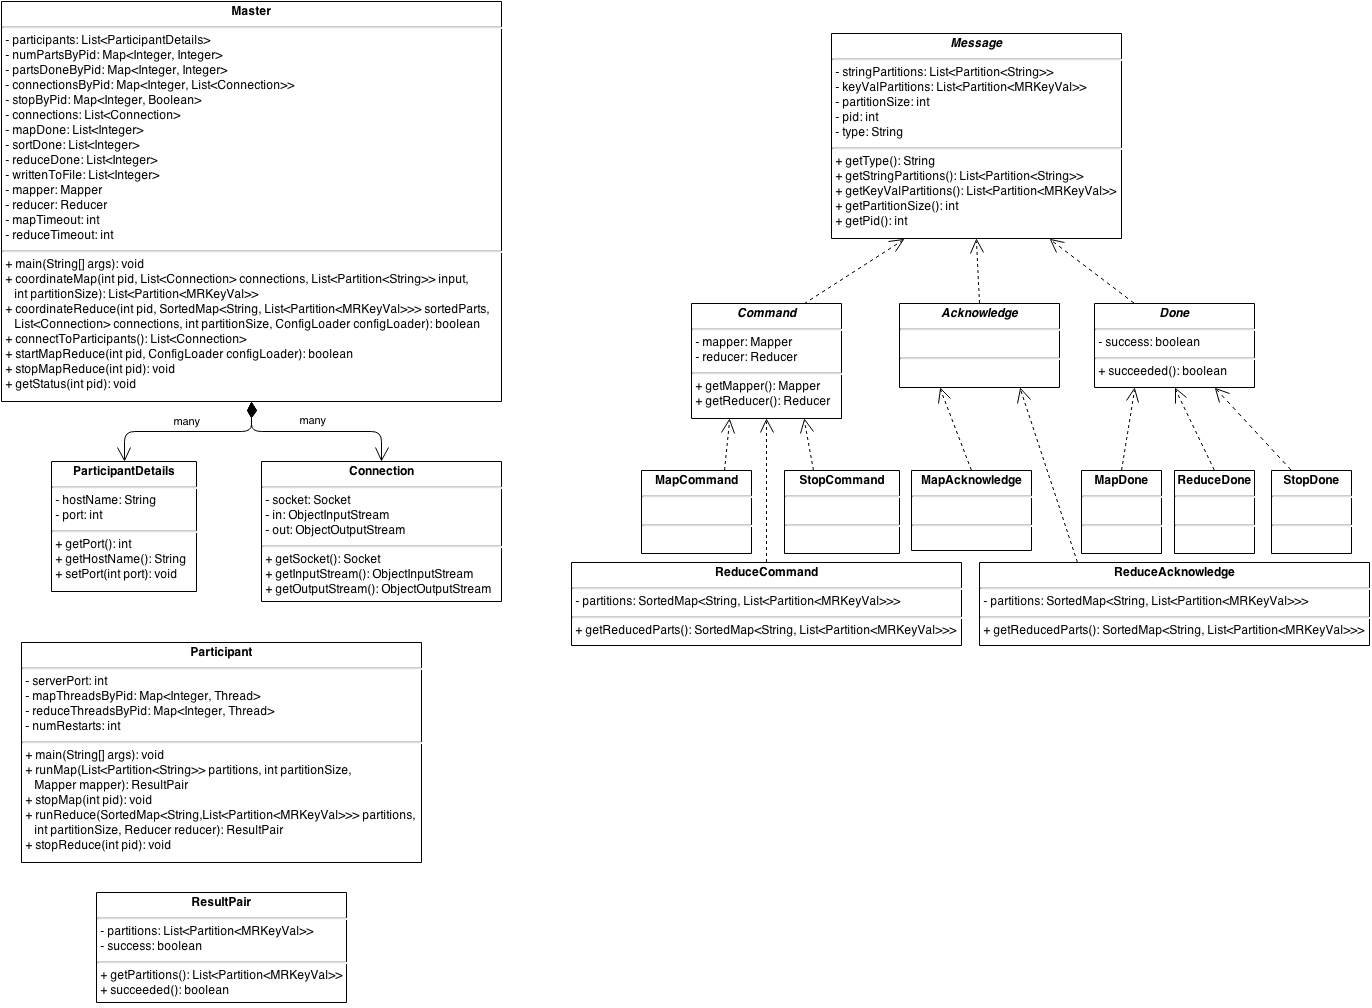
\includegraphics[scale=.35]{MapReduce_UML.png}

\subsubsection{UML Diagram of File IO}
File IO is composed of a \ttt{FileServer} that runs on all machines to serve the various map reduce partitions and \ttt{Partition}s and their associate supporting objects. The \ttt{Partition} forms the backbone of this system as it contains all of the key-value pairs in map reduce as well as serving to hold the initial input data once parsed from the input file. \ttt{RemoteFile} provides the functionality to interface with the \ttt{FileServer} and load remote files to the local machine. The \ttt{PartitionWriter} writes values to a partition until that partition reaches max size and then starts writing to a new partition. The \ttt{KeyPartitionWriter} takes this process to the next level by also storing partitions by key. 

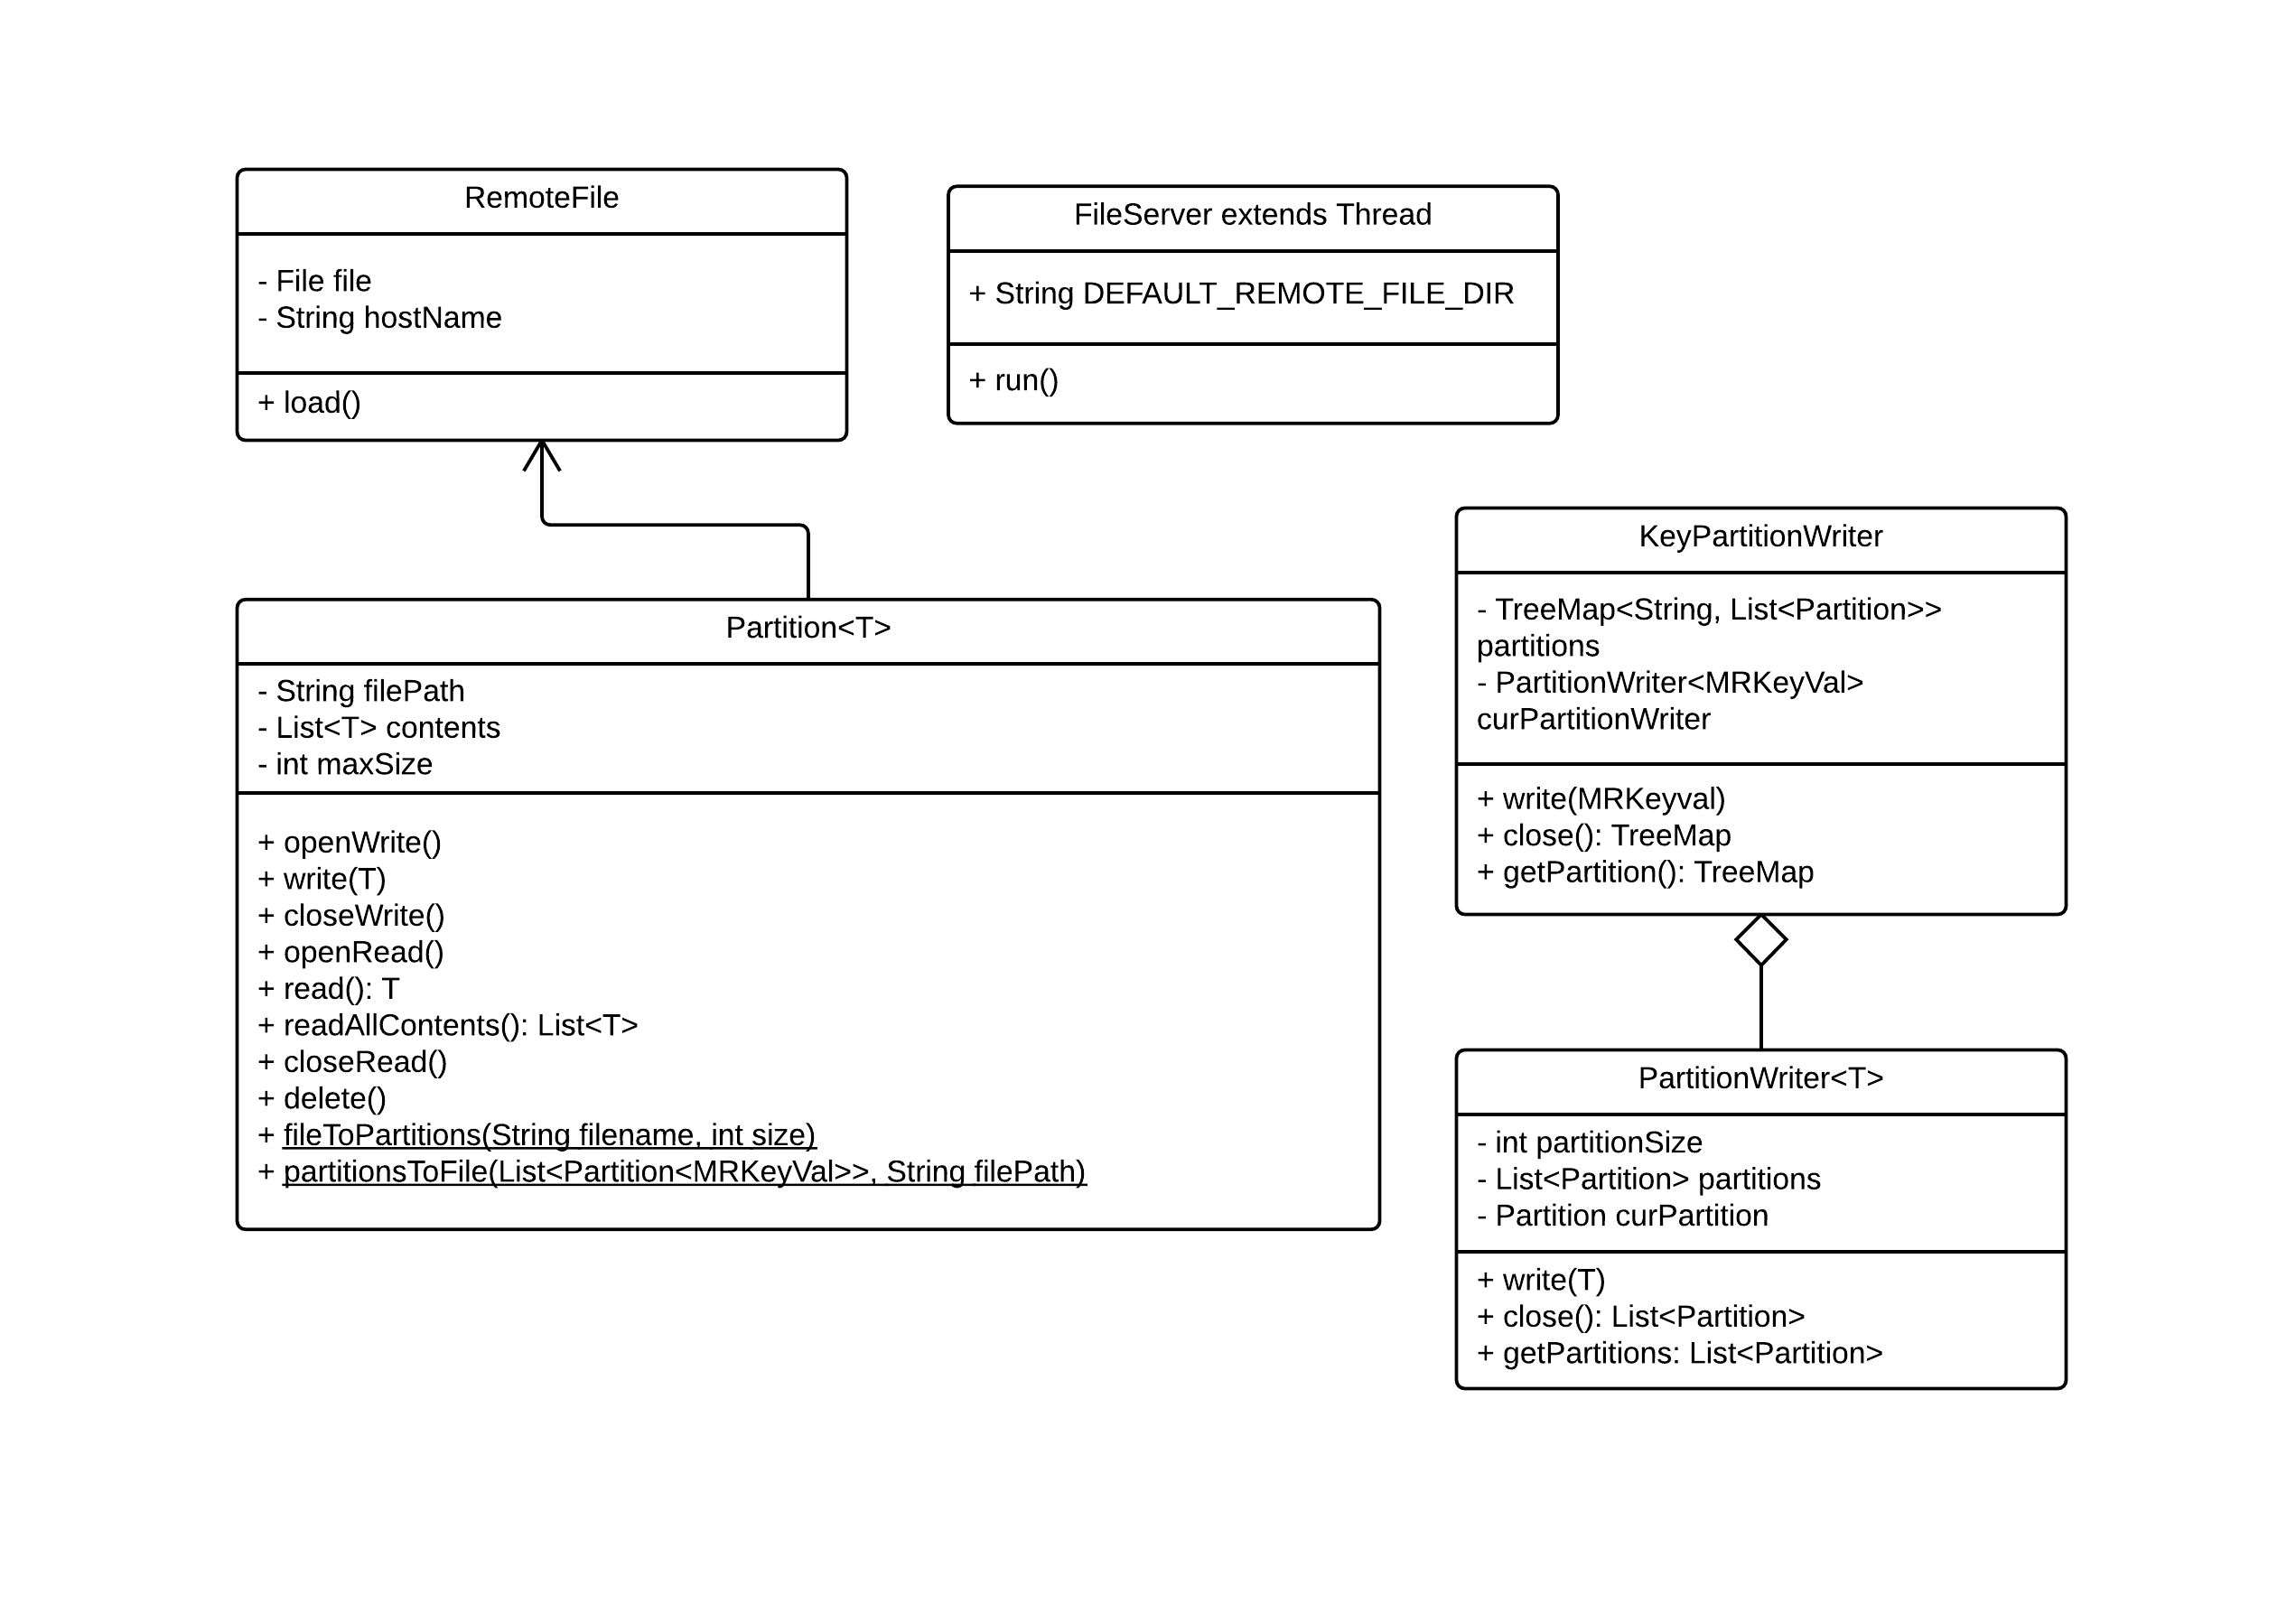
\includegraphics[scale=.7]{MapReduceFileIO_UML.png}

\subsubsection{UML Diagram of Map and Reduce Functions}
These are the objects which handle the basic map and reduce operations. \ttt{MapFn} and \ttt{ReduceFn} are the interfaces utilized by the application developer. All intermediate data in the map reduce system is stored as \ttt{MRKeyVal} which are string-integer key-value pairs.

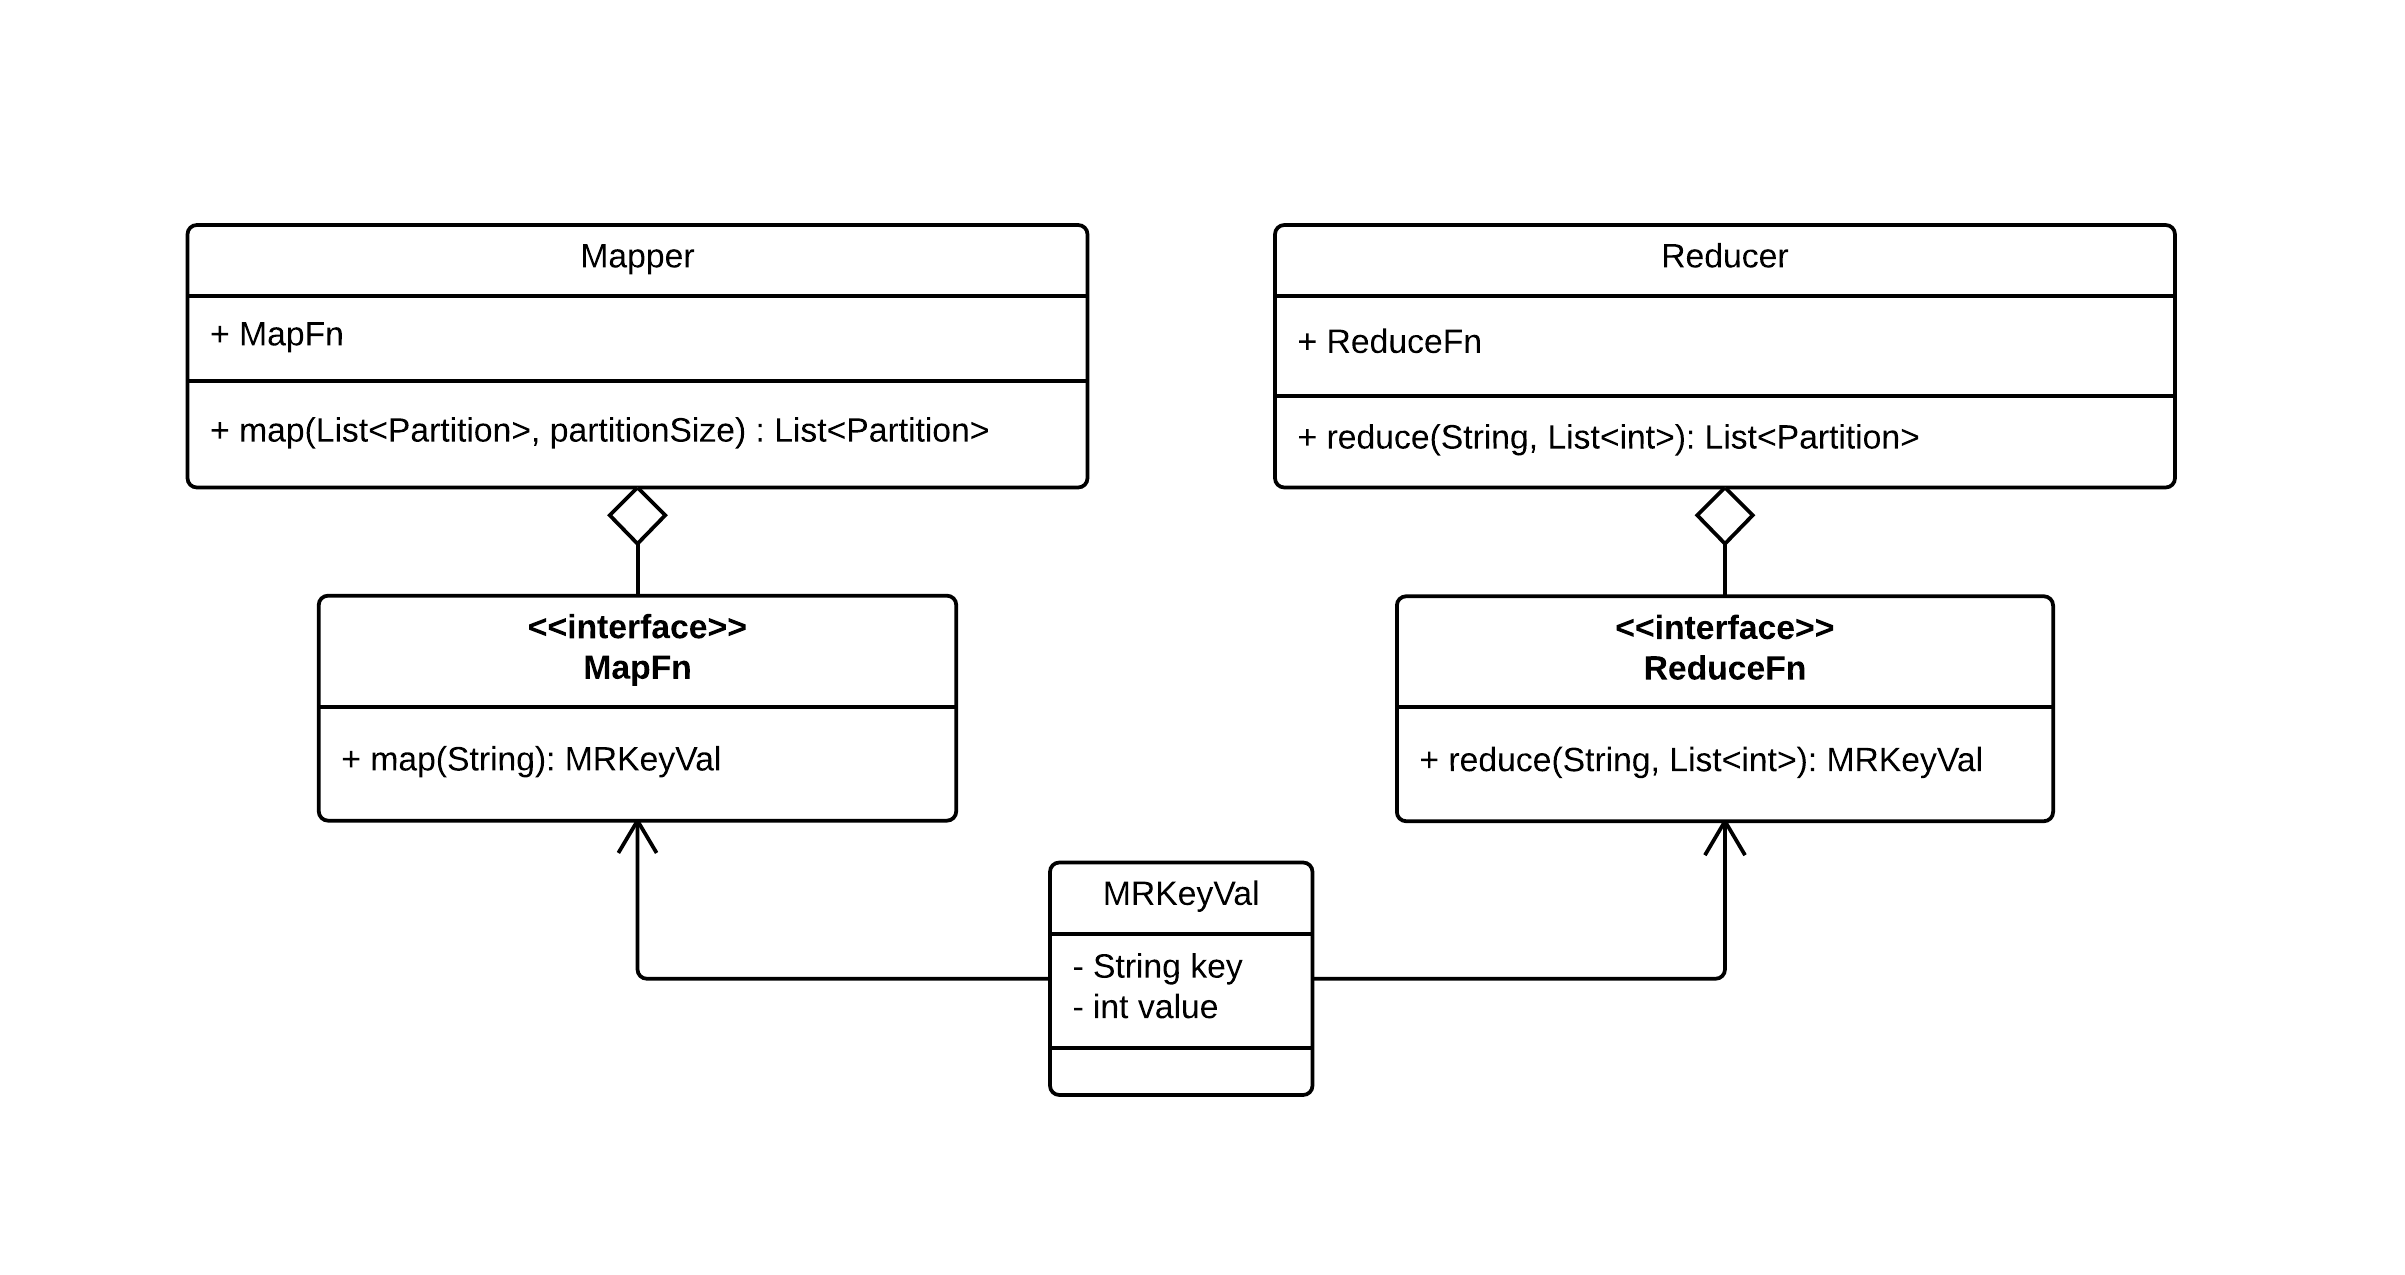
\includegraphics[scale=.7]{MapReduceFN_UML.png}

\subsubsection{Flow Diagram for user input `\ttt{start <config file>}'}
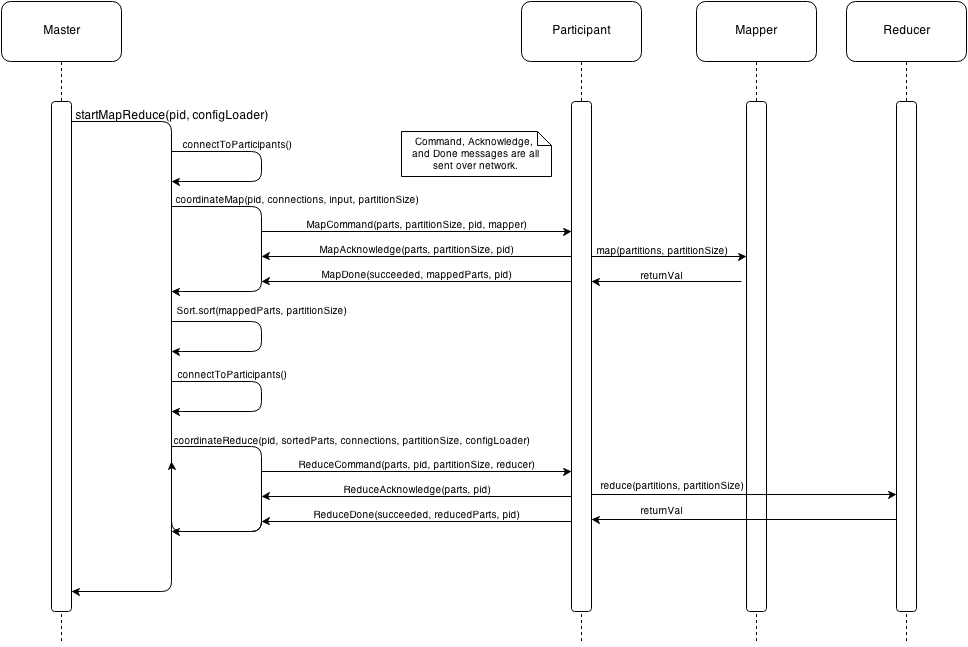
\includegraphics[scale=.5]{MapReduce_start.png}

\subsubsection{Flow Diagram for user input `\ttt{stop <pid>}'}
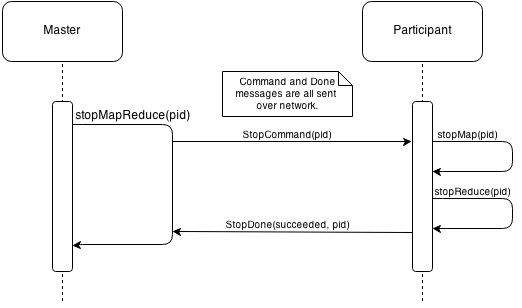
\includegraphics[scale=.7]{MapReduce_stop.png}

\subsection{Requirements Not Met and Limitations}

One fairly important limitation of our MapReduce facility as it currently stands is that due to the way in which we run the FileServer. Two participant nodes cannot be run on the same machine as they would both use the same file server port.

Another major limitation is that we rely on key value pairs of string and integer only. This can be easy extended to support generic types for key value pairs but as it stands currently the application developer is limited by this decision.

Beyond that, our MapReduce facility essentially functions as it is intended to. All standard processes work as designed. In the event of participant failure or Mapper/Reducer failure, any participants that are not working properly are disconnected and removed from the working list of participants (which defines where map/reduce partitions can be sent) and any failed partitions are retried on functional participants. Furthermore, all other unexpected failures (such as network problems, missing files, etc.) are handled in such a way that the user receives relevant, concise information about the failure and the Master and Participant code continue to run as they should (in other words, errors are handled cleanly and do not accidentally cause the entire Master or Participant code to abort).

\subsection{Improvements}

There is always room for improvement, and our MapReduce facility is no exception. We could provide support for map reduce key values of arbitrary types instead of just strings and integers. String-integer key pairs are enough to demonstrate the functionality of map reduce but it would be nice to allow other object types.

Additionally a full distributed file system would be helpful where files are backed up is a more distributed fashion on multiple machines instead of relying upon the master to always be the common source for files once a map reduce operation has completed. Our file system only distributes files during the map-reduce operation but does not create replicas of the output files.

\end{document}
